\documentclass[12pt]{article}

\usepackage[latin1]{inputenc}
\usepackage{amssymb}
\usepackage{amsmath}
\usepackage{amsthm}
\usepackage{bbold}
\usepackage{latexsym} 
\usepackage{graphicx}
\usepackage{bm}  
\usepackage{overpic} 
\usepackage[normalem]{ulem}
\usepackage{placeins}
\usepackage{multirow}
\usepackage{float}
\usepackage{url}
\usepackage{hyperref}
  
\usepackage{exscale}
\usepackage{amsfonts}
\usepackage[usenames,dvipsnames]{color} % load color package

\textwidth=6.0in \textheight=8.8in \hoffset=-0.2in
\voffset=-0.85in
\parskip=6pt
\baselineskip=9pt
\topmargin 0.8in
 
\def\black#1{\textcolor{black}{#1}}
\def\blue#1{\textcolor{blue}{#1}}
\def\red#1{\textcolor{red}{#1}}
\def\green#1{\textcolor{green}{#1}}
\def\yellow#1{\textcolor{yellow}{#1}}
\def\orange{\textcolor{BurntOrange}}

\newtheorem{definition}{Definition}[section]
\newtheorem{lemma}{Lemma}[section]
\newtheorem{remark}{Remark}[section]
\newtheorem{example}{Example}[section]
\newtheorem{theorem}{Theorem}[section]
\newtheorem{cor}{Corollary}[section]
\newtheorem{corollary}{Corollary}[section]

\numberwithin{equation}{section}

\newcommand{\E}{\mathbb{E}}
\newcommand{\R}{\mathbb{R}}
\newcommand{\sigl}{\sigma_L}
\newcommand{\BS}{\rm BS}
\newcommand{\p}{\partial}
\newcommand{\var}{{\rm var}}
\newcommand{\cov}{{\rm cov}}
\newcommand{\beaa}{\begin{eqnarray*}}
\newcommand{\eeaa}{\end{eqnarray*}}
\newcommand{\bea}{\begin{eqnarray}}
\newcommand{\eea}{\end{eqnarray}}
\newcommand{\ben}{\begin{enumerate}}
\newcommand{\een}{\end{enumerate}}
\newcommand{\quotes}[1]{``#1''}

\def\cC{\mathcal C}
\def\cD{\mathcal D}
\def\cS{\mathcal S}
\def\cH{\mathcal H}
\def\cI{\mathcal I}
\def\cJ{\mathcal J}
\def\cL{\mathcal L}
\def\cV{\mathcal V}
\def\cR{\mathcal R}
\def\bR{\mathbb R}
\def\cX{\mathcal X}
\def\cF{\mathcal F}
\def\bP{\mathbb P}
\def\bE{\mathbb E}
\def\bN{\mathbb N}
\def\bT{\mathbb T}
\def\bC{\mathbb C}
\def\var{\text{var\,}}
\def\eps{\varepsilon}
\def\bsq#1{\lq{#1}\rq}

\newcommand{\mt}{\mathbf{t}}
\newcommand{\mS}{\mathbf{S}}
\newcommand{\tC}{\widetilde{C}}
\newcommand{\hC}{\widehat{C}}
\newcommand{\tH}{\widetilde{H}}
\renewcommand{\O}{\mathcal{O}}
\newcommand{\dt}{\Delta t}
\newcommand{\tr}{{\rm tr}}

\begin{document}



\title{\bf An alternative approach to Black Litterman}

\author{Yixiang Wang\footnote{{\tt  yixiang.wang.ny@gmail.com}}{\setcounter{footnote}{1}} , Yue Wang\footnote{{\tt jasonyuewang@gmail.com}}{\setcounter{footnote}{2}} \thanks{Special thanks to our professor Gordon Ritter.}
}

%\date{This version: Nov 28, 2016}


\maketitle\thispagestyle{empty}
 
%%***************************************************************************
%%
%%  Document begins here
%%
%%***************************************************************************


%\usepackage{enumitem}
\begin{abstract}
In this report, we provided a generalized form of Black Litterman by showing explicitily how one would combine multiple views of factor returns on each single factor under APT model framework. Along with the form, we applied a variety of techniques to forecast factor returns and assessed its impact in this framework. 

% Inspired by the precedent work done by Petter Kolm and Gordon Ritter on their Bayesian Interpretation of Black Litterman.We present the most general model of the type considered by Black and Litterman (1991) after fully clarifying the duality between Black-Litterman optimiza- tion and Bayesian regression. Our generalization is itself a special case of a Bayesian network or graphical model. As an example, we work out in full detail the treatment of views on factor risk premia in the context of APT. We also consider a more spec- ulative example in which the portfolio manager specifies a view on realized volatility by trading a variance swap. 
\end{abstract}

%%%%%%%%%%%%%%%%%%%%%%%%%%%%%%%%%%%%%%%%%%%%%%%%%%%%%%%%%%%%%%%%%%%%%%%%%%%%%%%%%
%
%
%  Section: Introduction
%
%
%%%%%%%%%%%%%%%%%%%%%%%%%%%%%%%%%%%%%%%%%%%%%%%%%%%%%%%%%%%%%%%%%%%%%%%%%%%%%%%%%%

\section{Introduction}

% \subsection{Organization of the paper}
In this study, we conclude that the simplest EWMA-like Holt winter approach is the most appealing single filter to forecast the factor returns that yield an IR of 1.92 within Black Litterman framework applied in this dataset.The remainder of the paper is organized as follow: section 2 discusses the theoretical foundation for the Black Litterman model construction and associated mathematics. Section 3 describes the data and assumption and methodologies used to generate the result. Section 4 show the main results. Section 5 explores the behavior of the associated results and concludes.


\section{Theoretical Foundations}
\subsection{Overview of APT Model}

Multi-factor models assume a linear functional form
\begin{align} 
R_{t+1} = X_t f_t +\epsilon_t, \mathbb{E}[R_t]=0, \mathbb{V} [R_t]=D 
\end{align}
where $R_{t+1} $ is an n-dimensional random vector containing the cross-section of returns in excess of the risk-free rate over some time interval [t, t + 1], $X_t $is a (non-random) n x p matrix that is known before time t. Also $\epsilon_t$ is assumed to follow a mean-zero distribution with diagonal variance- covariance matrix
\begin{align} 
D := diag( \sigma_1^2,...,\sigma_n^2) \ with \  all \   \sigma_i^2 > 0.
\end{align}
Eq(1.2) entails that all significant sources of correlation are already cap- tured by factors, represented as columns of Xt. We henceforth suppress the implicit time index since most of our discussions concern a single time interval. Note, for later use, that $D^{-1}$ exists and can be computed in O(n) time.
The variable f in (2.1) denotes a p-dimensional random vector process which cannot be observed directly; information about the f-process must be obtained via statistical inference. We assume that the f-process has finite first and second moments given by
\begin{align} 
E[f] = \mu_f, \ and \ V[f] = F 
\end{align}

The primary outputs of a statistical inference process are the parameters
f and F mentioned in (3.3), and other outputs one might be interested in
include estimates of the daily realizations $\hat {f_t}$.

\subsection{Overview of Generalized Black Litterman Framework}

A Black-Litterman-Bayes model consists of:
\begin{itemize}
  \item  A parametric statistical model for asset returns $p(r\mid\theta)$ with finite-dimensional parameter vector.
  \item  A prior $ \pi $ on the parameter space.
  \item  A likelihood function $f(q\mid\theta)$ where $\theta$ is any parameter vector appearing in a parametric statistical model for asset returns, and q is a vector supplied by portfolio managers or economists.
  \item  A utility function u(w) of final wealth in the sense of Arrow(1971) and Pratt(1964).
\end{itemize}

Given a Black-Litterman-Bayes (BLB) model, the associated BLB optimal portfolio is defined to be 
\begin{align} 
h^* \in  \arg\max_{}  \E[u(\textbf{h}'\textbf{r}\mid \textbf{q})]
\end{align}
where $\E[ . \mid q]$ denotes the expectation with respect to the posterior predictive density for the random variable r. In other words, $h^*$ maximizes posterior expected utility.
\begin{align} 
p(r \mid q)&= \int p(r \mid \theta)\,p(\theta \mid q)\,d\theta \ \ where \\ 
p(\theta \mid q)&= \frac{p(q\mid \theta) \pi(\theta)}{\int p(q\mid \theta)\,\pi(\theta)\,d\theta}
\end{align}

Given a benchmark portfolio with holdings $\textbf{h}_B$ (eg. the market portfolio), and given a Black-Litterman-Bayes model (given above), the prior $\pi(\theta)$ is said to be benchmark-optimal if $\textbf{h}_B$ maximizes expected utility of wealth, where the expectation is taken with respect to the a priori distribution on asset returns $p(r)=\int p(r \mid \theta)\ \pi(\theta) d\theta$ so
\begin{align} 
h \in  \arg\max_{h}  \int u(\textbf{h}'\textbf{r})p(\textbf{r}\mid\theta)d\theta \
\end{align}

In summary, The model of Black and Litterman (1991) is the special case in which $r \mid \theta$ is multivariate normal with mean $\theta$ and $f(\ \mid \ )$ is the normal likelihood for a regression of the portfolio manager's views,the utility of final wealth is the CARA function $u(w) = -e^{-\delta w}$, and the prior is the unique normal distribution which is benchmark-optimal with respect to the market portfolio.

\subsection{Mathematics behind Black Litterman Portfolio Construction}
Starting with some views:
\begin{align} 
\E[\textbf{Pr}] &= \textbf{q} 
\end{align}
views serve as the noisy observations about r that statistical inference would be performed against
\begin{align} 
\textbf{r} \sim N(\boldsymbol{\theta}, \boldsymbol{\Sigma})
\end{align}

To represent its noisy property, we specify uncertainty associated with the view that expressed
\begin{align} 
\textbf{P} \boldsymbol{\theta} = \textbf{q} + \boldsymbol{\epsilon}^{(v)},\ \boldsymbol{\epsilon}^{(v)} \sim N(0, \boldsymbol{\Omega}) , \ \boldsymbol{\Omega} = diag(w_1, w_2, ..., w_k)
\end{align}

The noise is repesented by $\boldsymbol{\epsilon}^{(v)}$
The intuition behind this is if any random variable r comes from a density $p(r \mid \theta)$ with parameter $\theta$, and if one were given a set of noisy observations of realizations of r, then one could infer something about $\theta$ by statistical inference
To conduct statistical inference, not only one would need obeservations, but also a fully specified statistical model, which includes both prior and likelihood. 
based on the above definition, the likelihood is given as follows:
\begin{align} 
f(\textbf{q} \mid \boldsymbol{\theta}) \propto  exp[-\frac{1}{2}(\textbf{P}\boldsymbol{\theta}-\textbf{Q})^{'}\boldsymbol{\Omega}^{-1}(\textbf{P}\boldsymbol{\theta}-\textbf{Q})]
\end{align}
which essentially is a standard normal for a multiple linear regression with dependant variables $\textbf{q}$ and design matrix $\textbf{P}$
In the absence of any sort of information/views which could constitute alpha over the benchmark, the optimization procedure shouldsimply return the global CAPM equilibrium portfolio, with holdings denoted $\textbf{h}_{eq}$
\begin{align}
\textbf{r} \sim N(\boldsymbol{\theta}, \boldsymbol{\Sigma}) \ and \ \boldsymbol{\theta} \sim N(\boldsymbol{\Pi}, \textbf{F}) \\
\mathbb{E}[\textbf{p}^{'}\textbf{r}] = \textbf{P}^{'}\boldsymbol{\Pi} \ and \ \mathbb{V}[\textbf{p}^{'}\textbf{r}] = \textbf{p}^{'}(\boldsymbol{\Sigma}+ \textbf{C})\textbf{p}
\end{align}
We also need to make a choice whether to use the conditional or unconditional variance in optimization: 
equally:
\begin{align}
\mathbb{V}[\textbf{r}\mid\boldsymbol{\theta}] &= \boldsymbol{\Sigma} \ \textbf{v.s.} \ \mathbb{V}[\textbf{r}] = \boldsymbol{\Sigma} + \textbf{C}
\end{align}
In this case, we are concerned with unconditional variance i.e.  $\mathbb{V}[\textbf{r}] = \boldsymbol{\Sigma} + \textbf{C}$
Denote $\textbf{h} \in \mathbb{R}^{n}$ as the vector of portfolio holdings, which has \textbf{unit of dollars}. Mean Variance optimization will a risk-aversion parameter $\epsilon > 0$ leads to
\begin{align}
\textbf{h}_{eq} &= \epsilon^{-1}(\boldsymbol{\Sigma}+\textbf{C})^{-1}\boldsymbol{\Pi}
\end{align}
In a special case where $\textbf{C} = \tau \boldsymbol{\Sigma}$ with some scalar $\tau$ we will have 
\begin{align}
\textbf{h}_{eq} &= \epsilon^{-1}(1+\tau)\boldsymbol{\Sigma}^{-1}\boldsymbol{\Pi}
\end{align}

\noindent
we obtain the log posterior as following:
\begin{align}
(\textbf{P}\boldsymbol{\theta}-\textbf{Q})^{'}\boldsymbol{\Omega}^{-1}(\textbf{P}\boldsymbol{\theta}-\textbf{Q}) + (\boldsymbol{\theta}-\boldsymbol{\Pi})^{'}\textbf{C}^{-1}(\boldsymbol{\theta}-\boldsymbol{\Pi}) \\
= \boldsymbol{\theta}^{-1}[\textbf{P}^{'}\boldsymbol{\Omega}^{-1}\textbf{P} + \textbf{C}^{-1}]\boldsymbol{\theta} -2(\textbf{q}^{'}\boldsymbol{\Omega}^{-1}\textbf{P} + \boldsymbol{\Pi}^{'}\textbf{C}^{-1})
\end{align}
"completing the square" Lemma:
If a multivariate normal random variable $\boldsymbol{\theta}$ has density $p(\boldsymbol{\theta})$ and
\begin{align}
  -2 \log p(\boldsymbol{\theta}) &= \boldsymbol{\theta}^{'} \textbf{H} \boldsymbol{\theta} - 2 \boldsymbol{\eta}^{'}\boldsymbol{\theta} + term (\ without \ \boldsymbol{\theta})
\end{align}
then $\mathbb{V}[\boldsymbol{\theta}] = \textbf{H}^{-1}$ and $\mathbb{E}[\boldsymbol{\theta}] = \textbf{H}^{-1}\boldsymbol{\eta}$.
By above lemma: with $\textbf{H} =\textbf{P}^{'}\boldsymbol{\Omega}^{-1}\textbf{P} + \textbf{C}^{-1}$
the posterior has \textbf{mean}
\begin{align}
\textbf{v} &= [\textbf{P}^{'}\boldsymbol{\Omega}^{-1}\textbf{P} + \textbf{C}^{-1}]^{-1}[\textbf{P}^{'}\boldsymbol{\Omega}^{-1}\textbf{q} + \textbf{C}^{-1}\boldsymbol{\Pi}]
\end{align}
and \textbf{covariance} 
\begin{align}
\textbf{H}^{-1} &= [\textbf{P}^{'}\boldsymbol{\Omega}^{-1}\textbf{P} + \textbf{C}^{-1}]^{-1}
\end{align}
Based on CARA utility, equivalently to solve the following:
\begin{align}
\textbf{h}^{\textbf{*}} \in  \arg\max_{\textbf{h}}  \{ \mathbb{E}[\textbf{h}'\textbf{r}] - (\delta/2)\mathbb{V}[\textbf{h}'\textbf{r}] \}
\end{align}
where $\mathbb{E}[\textbf{r}]$ and $\mathbb{V}[\textbf{r}]$ represent \textbf{unconditional mean} and \textbf{covariance} of $\textbf{r}$ under the posterior.
we have the \textbf{variance} term can be represented as following:
\begin{align}
\mathbb{V}[\textbf{h}^{-1}\textbf{r}] &= \textbf{h}^{'}[\textbf{P}^{'}\boldsymbol{\Omega}^{-1}\textbf{P} + \textbf{C}^{-1}]^{-1}\textbf{h} + \textbf{h}^{'}\boldsymbol{\Sigma}\textbf{h}
\end{align}
and optimal portfolio holding is then
\begin{align}
\textbf{h}^{*} &= \delta^{-1}[\textbf{H}^{-1} + \boldsymbol{\Sigma}]^{-1}\textbf{H}^{-1}[\textbf{P}^{'}\boldsymbol{\Omega}^{-1}\textbf{q} + \textbf{C}^{-1}\boldsymbol{\Pi}]
\end{align}
where $[\textbf{H}^{-1} + \boldsymbol{\Sigma}]^{-1}$ is the updated \textbf{covariance} and $\textbf{H}^{-1}[\textbf{P}^{'}\boldsymbol{\Omega}^{-1}\textbf{q} + \textbf{C}^{-1}\boldsymbol{\Pi}]$ is the updated \textbf{mean}

\subsection{Step by Step Black Litterman Portfolio Construction}
\indent
Step 1 involves of calculate the posterior distribution of $\boldsymbol{\theta}$, after the view being taken into account, based on the assumption, the posterior distribution is of the same distributional family as the prior (again normal) - but with different parameters
If original parameters are $\boldsymbol{\xi}, \textbf{V}$ i.e. $\pi(\boldsymbol{\theta}) \propto N(\boldsymbol{\xi},\textbf{V})$
Then the updated parameters are:
\begin{align} 
\tilde{{\boldsymbol{\xi}}} &= (\textbf{V}^{-1} + \boldsymbol{\Omega}^{-1})^{-1} (\textbf{V}^{-1}\boldsymbol{\xi} + \boldsymbol{\Omega}^{-1} \textbf{q}) \\
\tilde{\textbf{V}} &= (\textbf{V}^{-1} + \boldsymbol{\Omega}^{-1})^{-1}
\end{align}
Step 2 follows similar calculation by using the updated values $\boldsymbol{\xi}, \textbf{V}$ we can find explicitly find the $\mathbb{V}[\textbf{r}\mid\boldsymbol{\theta}]$ and $\mathbb{E}[\textbf{r}\mid\boldsymbol{\theta}] $ (The explicit formula is omitted here)
Step 3 involves solve it in mean variance framework, but also substitution we can obtain the updated porftolio as following:
\begin{align} 
\textbf{h} &= \delta^{-1} \boldsymbol{\Sigma}^{-1}  \boldsymbol{\Pi} \\
\boldsymbol{\Pi} & := \textbf{X}\tilde{\boldsymbol{u}}_f \\
\tilde{\boldsymbol{u}}_f & := (\textbf{V}^{-1}+ \boldsymbol{\Omega}^{-1}+\textbf{X}^{'}\boldsymbol{\Sigma}^{-1}\textbf{X})^{-1}(\textbf{V}^{-1}\boldsymbol{\delta} + \boldsymbol{\Sigma}^{-1}\textbf{q})
\end{align}

\section{Main result}
\subsection{Data}
For this projcet, we study the United States equity market over the period 2006-2015 through the lens of an APT model. For each day t in our sample, we take n = 2000 and select the top n stocks in the US market, sorted by market capitalization. We chose this value because stocks falling below the top 2000 by market cap tend to be illiquid and have wide spreads, making them diffcult to trade for institutional investors. We restrict the study to common stock, hence excluding closed-end funds, REITs, ETFs, unit trusts, depository receipts, warrants, etc. Our only data sources for this study were CRSP and IBES which we access via the Wharton Research Data Service. 

We construct our model to contain five of the most commonly-studied and well-known sources of systematic risk: market beta, size, value, momentum, and volatility, as well as a classification of the stocks into industries.
some interpretation of the risk factors:

\begin{itemize}
  \item Market beta: each asset's daily excess return time series is winsorized and regressed against the SPX, over a 2-year window w   intercept. The beta is the slope coe cient. The results are further improved using the Vasicek (1973) Bayesian adjustment in the cross section.
  \item Size: market capitalization.
  \item Volatility: as in the market beta calculation, each asset's daily excess return time series is winsorized and regressed against          the SP 500 excess return time series, over a trailing two year window. The mean-square error (MSE) from this regression is the           raw exposure.
  \item Momentum: trailing compound returns over the last 12 months with the last 1 month excluded. 
  \item Value: the raw exposure is et/pt where et represents the sum of the trailing 4 quarters' earnings-per-share (EPS), adjusted for          splits, and pt is the close price on day t.
\end{itemize}

\subsection{Assumption}
The study presented in this paper heavily relies on the prior ground-breaking work that has been done by Peter Kolm and Gordon Ritter in their paper.

Within APT, the factor $f$ could be well defined by its first and second moment,
(when $f$ has a finite first and second moment) we could induce the following:
\begin{align} 
\E[{\bf f}] =  \boldsymbol{\mu}_f, V[{\bf f}] = \textbf{F}
\end{align}
which leads to a further reduction of the following:
\begin{align} 
\E[{\bf f}] =  \boldsymbol{\mu}_f,  \boldsymbol{\Sigma} := V[{\bf f}] = \textbf{D} + \textbf{X} \textbf{F} \textbf{X} '
\end{align}
Back to the black litterman, we are free to choose $\boldsymbol{\theta}$ (the distribution of prior $\boldsymbol{\theta}$) as any vector of parameters appearing in a parametric statistical model for asset returns; It seems to be natural to choose $\boldsymbol{\theta}= u_f$ , the \textbf{k} parameters describing the factor risk premia. For simplicity we treat \textbf{F} as a constant matrix, just as the original Black-Litterman model treats $\boldsymbol{\Sigma}$ as a constant matrix.

Define the likelihood function to be (Normal likelihood again)
\begin{align} 
f(q \mid \theta) &= \prod_{i=1}^{k} exp[{-\frac{1}{2w_i^2}(\theta_i - q_i)^2}]
\end{align}
Conventionally, there are mainly two types of priors: one driven by historical data, and one driven by the desire to have some specific
benchmark turn out to be optimal under the model of the prior, in this paper we will solely address the first approach.
Residing on the nature of APT model, we applied an OLS approach to estimate the factor return cross-sectionally at any given t by 
introducing the data driven approach
  \begin{itemize}
    \setlength{\itemindent}{.25in}
    \item  random proecess driving $f$ is stationary implies $\boldsymbol{\mu}_f$ and ${\bf f}$ constant overtime
    \item  use simple OLS estimates  $f_t = (\textbf{X}_t ' \textbf{X}_t)^{-1} \textbf{X}_t' \textbf{r}_{t+1}$ to be prior mean
    \item  resulting model treat each time period as a "group" with $\textbf{r}_{t+1} \sim N(\textbf{X}_t \textbf{f}_t, \textbf{D})$ and $\textbf{f}_t$ modeled as i.i.d. draws $\textbf{f}_t \sim N(\textbf{u}_t, \textbf{F}) $
    \item  The statistical inference problem is then to infer $\boldsymbol{\theta} = \textbf{u}_f$ from obs of $\textbf{D}t$
  \end{itemize}
\setlength{\itemindent}{-.25in}
Note: The "data-driven" approach to prior selection that we have just described has the advantage of not requiring a benchmark portfolio. In particular, this makes sense for absolute return strategies where the elective benchmark is cash.
 
\subsection{Methodology and our approach}
\subsubsection{Estimation of factor returns and covariances}
Define the prior:
 \begin{itemize}
    \setlength{\itemindent}{.25in}
    \item  6-month lookback window
    \item  $\textbf{u}_f$ to be the mean of looking back window factor return
    \item  $\textbf{F}$ to be the covariance of looking back window factor return
    \item  $\textbf{D} := diag( \sigma_1^2,...,\sigma_n^2) \ with \  all \   \sigma_i^2 > 0$ via time series of cross sectional regression residual at each time t and average over based on initial looking back window
 \end{itemize}

\subsubsection{Market Portfiolio and Black Litterman Portfolio}
Based on the above assumptions, we will be able to derive the following results:
Market Portfolio:
\begin{align}
\textbf{F}_{mar} := (\delta \boldsymbol{\Sigma})^{-1}  \textbf{X}_t \textbf{u}_f, \ where \ \boldsymbol{\Sigma}_{t} = \textbf{X}_t \textbf{F}  \textbf{X}_t^{'} + \textbf{D}_t
\end{align}

Black Litterman Portfolio:
\begin{align}
\textbf{h}_{blb} &= \delta^{-1} \boldsymbol{\Sigma}^{-1} \textbf{X}(\textbf{V}^{-1}+ \boldsymbol{\Omega}^{-1}+\textbf{X}^{'}\boldsymbol{\Sigma}^{-1}\textbf{X})^{-1}(\textbf{V}^{-1}\boldsymbol{\delta} + \boldsymbol{\Sigma}^{-1}\textbf{q})
\end{align}
 
 
% Different from what has been done by Gordon in their paper, we dont explicitly determine the $\testbf{u}_f$ and $\textbf{F}$, instead just based on initial looking back windows.
\subsubsection{Generalized Black Litterman Portfolio}
Instead of presenting single view for each single factor (recall the likelihood define previously)
\begin{align} 
f(q \mid \theta) &= \prod_{i=1}^{k} exp[{-\frac{1}{2w_i^2}(\theta_i - q_i)^2}]
\end{align}

where specifically each i corresponding to a single view to a single factor with total of $\textbf{k}$ factors.

we proposed a transform of likelihood to be
\begin{align} 
f(q \mid \theta) &= \prod_{i=1}^{k}\prod_{j=1}^{n} exp[{-\frac{1}{2w_{ij}^2}(\theta_i - q_{ij})^2}]
\end{align}
where n is the number of views for each single factor

In black litterman, the optimal holding based on this construct will be instead 
\begin{align}
\textbf{h}_{blb} &= \delta^{-1} \boldsymbol{\Sigma}^{-1} \textbf{X}(\textbf{V}^{-1}+ \textbf{M}^{'}\boldsymbol{\Omega}^{-1}\textbf{M}+\textbf{X}^{'}\boldsymbol{\Sigma}^{-1}\textbf{X})^{-1}(\textbf{V}^{-1}\boldsymbol{\delta} +  \textbf{M}^{'}\boldsymbol{\Sigma}^{-1}\textbf{q})
\end{align}

Where $\textbf{M}$  are specified as following:
we can think orginally M is an identity matrix $\mathbb{1}_{n,n}$, now updated to a matrix for each factor, we have equal number of methods to forecast, say $\textbf{n}$ then its $\textbf{n}$ by $\textbf{k}$ matrix defined as following 
\begin{align}
\textbf{M} & =
\begin{bmatrix}
    x_{1,1}     & x_{1,2}     & x_{1,3}     & \dots  & x_{1, k} \\
    x_{2,1}     & x_{2,2}     & x_{2,3}     & \dots  & x_{2, k} \\
    \vdots      & \vdots      & \vdots      & \ddots & \vdots \\
    x_{n,1}     & x_{n, 2}    & x_{n, 3}    & \dots  & x_{n, k} \\
    x_{n+1,1}   & x_{n+1, 2}  & x_{n+1, 3}  & \dots  & x_{n+1, k} \\
    x_{n+2,1}   & x_{n+2, 2}  & x_{n+2, 3}  & \dots  & x_{n+2, k} \\
    \vdots      & \vdots      & \vdots      & \ddots & \vdots \\
    x_{2n, 1}   & x_{2n, 2}   & x_{2n, 3}   & \dots  & x_{2n, k} \\
    \vdots      & \vdots      & \vdots      & \ddots & \vdots \\
    x_{k(n-1)+1,1}   & x_{k(n-1)+1, 2}  & x_{k(n-1)+1, 3}  & \dots  & x_{k(n-1)+1, k} \\
    x_{k(n-1)+2,1}   & x_{k(n-2)+2, 2}  & x_{k(n-1)+2, 3}  & \dots  & x_{k(n-1)+2, k} \\
    \vdots      & \vdots      & \vdots      & \ddots & \vdots \\
    x_{kn, 1}   & x_{kn, 2}   & x_{kn, 3}   & \dots  & x_{kn, k}
\end{bmatrix}
=
\begin{bmatrix}
    1     & 0     & 0     & \dots  & 0 \\
    1     & 0     & 0     & \dots  & 0 \\
    \vdots      & \vdots      & \vdots      & \ddots & \vdots \\
    1     & 0    & 0    & \dots  & 0 \\
    0     & 1  & 0  & \dots  & 0 \\
    0     & 1  & 0  & \dots  & 0 \\
    \vdots      & \vdots      & \vdots      & \ddots & \vdots \\
    0     & 1   & 0  & \dots  & 0 \\
    \vdots      & \vdots      & \vdots      & \ddots & \vdots \\
    0   & 0  & 0  & \dots  & 1 \\
    0   & 0  & 0  & \dots  & 1 \\
    \vdots      & \vdots      & \vdots      & \ddots & \vdots \\
    0   & 0   & 0   & \dots  & 1
\end{bmatrix}
\end{align}

and $\boldsymbol{\Omega}$ to be diagonal matrix $\textbf{n}$ by $\textbf{k}$ to repesent the uncertainty in each speicific view by $(\textbf{i},\textbf{j})$ entry of the matrix - ith view about j-th factor.
\begin{align}
\boldsymbol{\Omega} & =
\begin{bmatrix}
    w_{11} &\hfill  &\hfill  &\hfill  &\hfill \\
    &\hfill w_{12}  &\hfill  &\hfill  &\hfill \\
    &\hfill &\ddots &\hfill  &\hfill \\
    &\hfill &\hfill &\hfill  w_{nk-1} &\hfill \\
    &\hfill &\hfill &\hfill  &\hfill  w_{nk}\\
\end{bmatrix}
\end{align}

To make computationally efficient, we make $\forall \ \textbf{j}, \textbf{i} \in (1,n)$, in another word, each factors we have exactly n views, this generalization however works for any j such that $\textbf{k}_{j_{m}} \neq \textbf{k}_{j_{n}}$ where  $m \neq n$

% \begin{table}[h]
% \begin{center}
%   \includegraphics{tableonedataclean}
%   \caption{Data Sample from \textit{OptionMetrics}}
%   \label{fig:one}
%   \end{center}
% \end{table}


% \FloatBarrier
% \begin{table}[h]
% \begin{center}
% \includegraphics{tabletwoafterclean}
%   \caption{Data Sample after cleaning}
%   \label{fig:two}
%   \end{center}
% \end{table}

\subsection{Factor Return Forecasting methods}
A core aspect of bayesian method or equivalently Black Litterman framework in our case is only as good as its input, which in the cases are really the views or the forecast of the factor returns namely $\textbf{q}_{i,t}$ we will mainly address three broad aspects of forecasting toolbox, namely simple MA filter, traditional statistical time series models as well as a particular machine learning technique named Recurrent Neural Networks

\subsubsection{Exponential Moving Average}
Without going into too much details (it's abundant in literature), we have three smoothed window with 5-days, 30-days and 120-days of half-life
\subsubsection{Traditional Time Series}
\begin{itemize}
  \setlength{\itemindent}{.25in}
  \item  Autoregressive integrated moving average(ARIMA) 
  \item  Holt Winter
  \item  Vectorized AutoRegression
\end{itemize}
All the above techniques, we applied an auto model and parameter selection that embedded in R or Python that based on either AIC or BIC criteria to select the best model to do the one day ahead forecast based on looking-back window data

\subsubsection{Machine learning with Recurrent Neural Network}
Recurrent Neural Network handles the information loss that encountered by traditional neural network to allow information to persist (It's unclear how a traditional neural network could use its reasoning about previous events to inform later ones)
\begin{itemize}
  % \setlength{\itemindent}{.25in}
  \item  Recurrent Neural Network(RNN)
    \begin{itemize}
      \item networks with loops
      \item can be thought as multiple networks and each passing a meassage to successsor
      \item ability to connect previous information to the present task
    \end{itemize}
  \item  Long Short Term Memory networks(LSTM Networks)
    \begin{itemize}
      \item a special kind of RNN 
      \item aimed to solve long term dependences as the gap between past and present widen where RNN might underperform
    \end{itemize}
  \item  Gated Recurrent Unit(GRU)
    \begin{itemize}
      \item a more dramatic variation - simpler than LSTM
      \item combines partial loss information into update, growing popularity
    \end{itemize}
\end{itemize}
From the existing studies, its unclear which version of RNNs works best.

\section{Main Results}
\subsection{IR of portflios}
Aside from the above-mentioned nine ways forecasting factor return, we also applied our generalized framework defined in 3.8 to combine some different return forecast mechanisms.\\
our IR (Note: here we directly use daily PnL as proxy of $\textbf{r}$) is defined as:
\begin{align}
\frac{\mathbb{E}(\textbf{r})}{\mathbb{V}(\textbf{r})} * Annualized \ Factor 
\end{align}
% below are the IR for different portfolios:
\begin{center}
\begin{tabular}{ |c|c|c|c| }
\hline
Period from 2006.05-2015 & Information Ratio \\
\hline
ARIMA & 1.65251310236 \\
GRU & 1.41910485371  \\
Holt Winters & 1.92422234646  \\
LSTM & 1.56851696395 \\
MA5 & 1.893804042  \\
Markowitz & 1.74641973298  \\
Simple RNN & 1.5712844355 \\
Simple RNN and MA5 & 1.90596235524  \\
VAR & 1.00522552586  \\
Multi-EMA & 1.65257029739  \\
\hline
\end{tabular}
\end{center}
Below is the cumulative PnL of the abover portfolios:

\begin{figure}[H]
  \begin{center}
  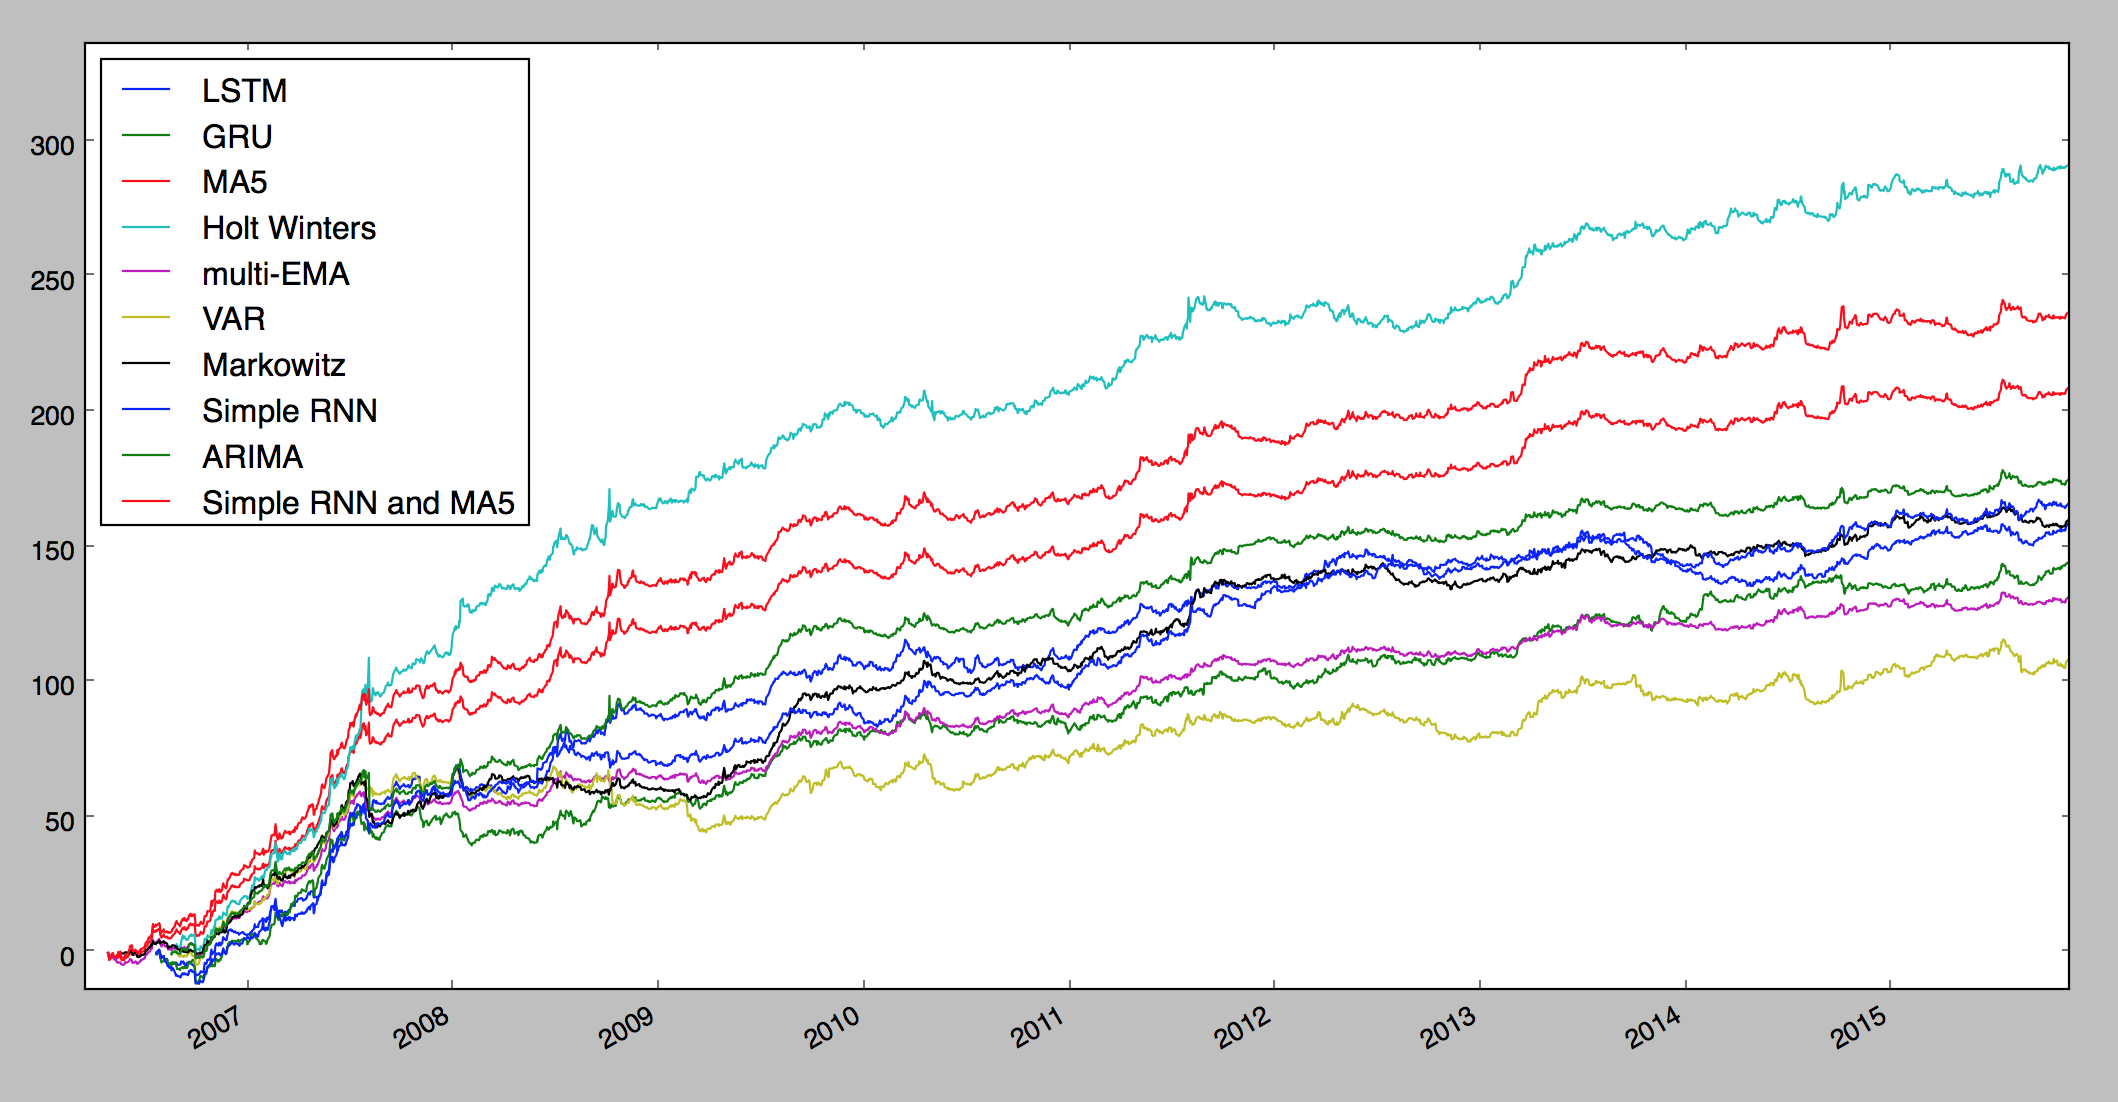
\includegraphics[width=\linewidth]{pnl_comparison.png}
  \caption{Cumulative PnL}
  \label{fig:1}
  \end{center}
\end{figure}

\subsection{Recap of proposed Generalized Framework}
\noindent
Remark: Given the time constraints, we applied genearalized framwork defined in (3.8) to the following:
\begin{itemize}
      \item combine different Exponential Moving Average windows 
      \item combine RNN with Exponential Moving Average short window
\end{itemize}
In practice, the generalized framework could applied any number of views, even in the case where number of views for each factor returns are different.


\section{Summary and conclusion}
In general, among of all the different strategies we applied in this study, all of them would be able to achieve an $IR>1$. With the worst performer being VAR and Top performer to be Holt Winter method. It is very surprising that the simplest short window moving average filter works really well which corresponds to the second best single alone strategy among the all. By blending multi views, we managed to achieved a better risk-adjusted performance as indicated by MA5 combined with RNN achieved a better IR than both RNN alone and MA5 alone, but the outperformance over MA5 is marginal. However,this blending method applied on multiEMA doesnt really beat MA5. Even more surprisingly, without any bayesian inference, the stand-alone historical average approach seems to be working well with IR of 1.75. This seems daunting as it doesent coincide with the result that presented by Gordon in their earlier paper, However, one needs to keep in mind that the dataset we applied is a shorter version of orginal study. we didnt explicitly assume a fator return and covariance, so the initial looking-back windows will impose a big impact on the performance of underlying Markowitze portfolio performance. In general, the performance of RNNs' family doesnt diff much which is relatively stable. As opposed to machine learning, the traditional time series have a divergent performance difference with ARIMA being mediocre.On the other hand, it entails us how sensitive the bayesian model would be to its posterior.

\section*{Acknowledgments}

We are very grateful to Professor Gordon Ritter

%%%%%%%%%%%%%%%%%%%%%%%%%%%%%%%%%%%%%%%%%%%%%%%%%%%%%%%%%%%%%%%%%%%%%%%%%%%%%%%%%%%%%%%%
%
%
%  Bibliography
%
%
%%%%%%%%%%%%%%%%%%%%%%%%%%%%%%%%%%%%%%%%%%%%%%%%%%%%%%%%%%%%%%%%%%%%%%%%%%%%%%%%%%%%%%%%

\begin{thebibliography}{}

\bibitem{Gordon Paper} 
Kolm, Petter N. and Ritter, Gordon
\textit{On the Bayesian Interpretation of Black-Litterman}. 
European Journal of Operational Research, Forthcoming, 2016.

\bibitem{GS} 
Guangliang He and Robert Litterman
\textit{The Intuition behind Black-Litterman Model Portfolios}. 
{Goldman Sachs Asset Management} (2006).

\bibitem{BL}
Satchell, Stephen, and Alan Scowcroft
\textit{A demystification of the Black-Litterman model:Managing quantitative and traditional portfolio construction}. 
{Journal of Asset Management 1.2, pp. 138-150} (2000).

@misc {RNN, author={Christopher, Olah},title = {{Understanding LSTM Networks}},
  howpublished="\url{http://colah.github.io/posts/2015-08-Understanding-LSTMs/}",
  year = {2015}, note="[Online; accessed 20-Dec-2016]"
}




\end{thebibliography}
\end{document}


